\chapter{Theoretische Betrachtung des REST Architekturstils}\label{chapter:theoretische-betrachtung}

Bei der Umsetzung einer Middleware zur REST Kommunikation stellt sich zunächst die erste Forschungsfrage nach dem Aufbau einer solchen REST Kommunikation. Der REST Architekturstil wird im Folgenden aus der Primärliteratur von Roy Fielding sowie anderer Fachliteratur herausgearbeitet und abstrahiert zusammengefasst:

\section{Quellendiskussion}\label{section:quellendiskussion}

Der REST Architekturstil wurde von Roy Fielding erfunden und zuerst in Fieldings Doktorarbeit “Architectural Styles and the Design of Network-based Software Architectures” beschrieben. Somit kann die Dissertation von Fielding als erste und wichtigste Primärquelle angesehen werden. Der REST Architekturstil ist eine Abstraktion des ebenfalls zu großen Teilen von Fielding konzipierten HTTP Protokolls . Somit sollte das HTTP Protokoll in der Fassung von 1999 auch als Primärquelle aufgenommen werden. Auch andere Request For Comments (RFC) der IETF werden als Primärquelle angesehen. 

Die Arbeit von Fielding befasst sich nicht mit der Umsetzung der Regel des REST Stils und auch nicht mit der Priorisierung dieser Regeln. Diese beiden Aspekte werden jedoch für diese Arbeit benötigt. Für diese Informationen wird auf Sekundärliteratur zurückgegriffen. 

\subsection{Quellen zur konkreten Umsetzung des REST Architekturstils}\label{subsection:qullen-zur-konkreten-umsetzung}

\begin{figure}[htb]
\centering
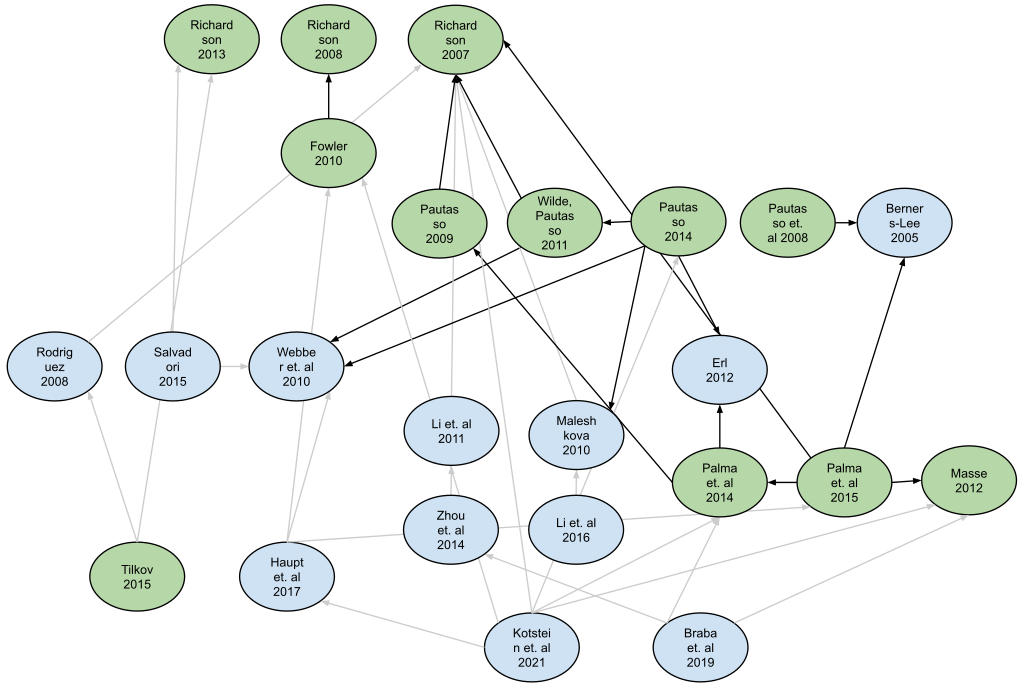
\includegraphics[width=\textwidth]{graphics/quelleneinordnung.png}
\caption[quelleneinordnung]{Quelleneinordnung}
\label{abb:QuellenEinordnung}
\end{figure}


Es wurde eine Vielzahl von Quellen untersucht. Diese Quellen sind in Abbildung .. aufgeführt. 

Die Kreise stellen die einzelnen Quellen dar. Ein Pfeil von Quelle A zu Quelle B symbolisiert eine Referenz von Quelle A auf Quelle B. Alle Quellen beziehen sich zusätzlich zu den hier aufgeführten Referenzen auf Roy Fieldings Doktorarbeit. Zur weiteren Synthese der Quellen wurde versucht, die Qualität der Quellen zu beurteilen. Alle als qualitativ beurteilten Quellen sind in der Abbildung in grün dargestellt. Diese werden in der folgenden Arbeit hauptsächlich verwendet. Die Beurteilung der Quellen wird im Folgenden begründet:

Zunächst werden die Quellen von Richardson von 2007, 2008 und 2013 betrachtet: Alle Quellen werden vielfach zitiert. Da andere Autoren ebenfalls auf die Auswahl hochwertiger Quellen achten sollten, lässt sich annehmen, dass eine viel zitierte Quelle von hoher Qualität ist. Gerade das Lehrbuch “RESTful Web Services” (2007) wurde besonders oft zitiert. Zusätzlich sind Richardsons Werke bei dem 1978 gegründeten, anerkannten Verleger O’Reilly publiziert. Weitergehend ist Leonard Richardson der Autor der populären  Bibliothek Beautiful Soup zum parsen von XML und HTML Dokumenten  und arbeitete bereits als Software Architekt bei der New York Public Library, sowie bei Canonical, der Firma hinter Ubuntu. Insgesamt wurden seine Werke über 1500 mal zitiert.

Auch die Werke von Pautasso wurden vielfach zitiert. Cesare Pautasso is full professor at the Software Institute of the Faculty of Informatics at the University of Lugano, Switzerland. Previously he was a researcher at the IBM Zurich Research Lab (2007) and a senior researcher at ETH Zurich (2004-2007). He completed his graduate studies with a Ph.D. from ETH Zurich in 2004 and his undergraduate studies at Politecnico di Milano, Italy with a Computer Science Engineering Degree (cum laude) in 2000.

Francis Palma wird ebenfalls als ein Spezialist auf seinem Fachgebiet angesehen und weißt einen h-Index von 12 auf. Seine Werke werden unter kritischer Betrachtung ebenfalls als Quellen aufgenommen.

Ein Lehrbuch von Mark Masse wird auch als Quelle aufgenommen. Masse verfügt über fünfzehn Jahre Erfahrung in Technik, Management und Architektur der Informatik und entwarf das Content Management System (CMS) von allen Websites der Walt Disney Company. Das vorliegende Lehrbuch ist jedoch teils subjektiv gehalten und sollte somit besonders kritisch hinterfragt werden.

Eine weitere betrachtete Quelle ist ein Lehrbuch von Stefan Tilkov. Das Lehrbuch wurde aufgrund einer mündlichen Empfehlung der Bibliothek der Dualen Hochschule Baden-Württemberg (DHBW) sowie der Universität Stuttgart ausgewählt. Auch ist Stefan Tilkov Berater bei INNOQ, Autor zahlreicher Fachartikel und Referent auf zahlreichen internationalen Konferenzen. Gleichzeitig wurde das Buch jedoch laut Google Scholar nur 15 mal zitiert. Aus diesem Grund wird es im Folgenden auch kritischer betrachtet.

\subsection{Quellen zur Priorisierung der Rest Regeln}\label{subsection:quellen-zur-priorisierung}

Johanna Barzen und Sebastian Kotstein erstellten eine Umfrage unter Experten, welche REST Regeln am wichtigsten sind. Die Meinungen dieser Experten werden auch in der Priorisierung der REST Regeln in dieser Arbeit berücksichtigt.

\section{Definitionen und Begriffe}\label{subsection:definitionen-und-begriffe}

Fielding legte bei der formulierung seines REST Architekturstil einen besonderen Fokus auf die Definition und korrekte Verwendung von speziellen Begriffen. Diese werden im folgenden zusammengefasst.

\subsection{Ressourcen und Repräsentationen}\label{subsection:ressourcen-und-repraesentationen}

Da es sich bei REST um einen Stil zur Umsetzung von verteilten Informationssystemen handelt, liegt es auf der Hand, zunächst die Modellierung von Informationen zu betrachten. Die Abstraktion einer jeden Information in REST stellt eine Ressource dar . Zu jedem Abfragezeitpunkt entspricht eine Ressource einem bestimmten Set von Ressourcen Repräsentationen und/-oder Ressourcen Metadaten. Ressourcen Repräsentationen sind konkrete Daten in einer konkreten Darstellungsform, wie zum Beispiel ein Bild oder ein Text  . Die Metadaten beschreiben diese Daten, sodass sie angemessen verarbeitet werden können.

\subsection{Verbindungselemente}\label{subsection:verbindungselemente}

Neben Ressourcen und Repräsentationen sieht die REST Architektur von Roy Fielding eine Reihe von Verbindungselementen vor. Er beschreibt Verbindungselemente als abstrakte und generalisierte Konstrukte zwischen den anderen Komponenten. Diese abstrakte Betrachtung der Verbindungselemente hat den Vorteil, dass die Komponenten des Netzwerkes, wie z.B. der Client und der Server keine konkreten Informationen über die Implementierung der Verbindungselemente benötigen, so lange sie ebenfalls dem einheitlichen Protokoll folgen. Der generische Aufbau eines Verbindungselementes wird in der folgenden Abbildung gezeigt:

Die Schnittstelle des Verbindungselementes ähnelt dem prozeduralen Aufruf, jedoch mit einigen wichtigen Unterschieden: Die Eingangsparameter bestehen aus Anfragekontrolldaten, einer Ressourcenkennung, die das Ziel der Anfrage angibt, und einer optionalen Repräsentation. Die Out-Parameter bestehen aus Antwort-Kontrolldaten, optionalen Ressourcen-Metadaten und einer optionalen Darstellung. Aus abstrakter Sicht ist der Aufruf synchron, aber sowohl Eingangs- als auch Ausgangsparameter können als Datenströme übergeben und somit asynchron implementiert werden.

Die primären Verbindungselemente sind der Client und der Server. Der Unterschied zwischen beiden besteht darin, dass der Client eine Verbindungsanfrage initiiert und der Server diese Anfrage beantwortet. Die drei zuletzt genannten Verbindungselemente werden im Rahmen dieser Arbeit nicht weiter erläutert, da sie von geringer Relevanz für die implementierung der Middleware sind.

\subsection{Komponenten}\label{subsection:komponenten}

Ein Useragent verwendet das Client Verbindungselement, um Abfragen abzuschicken und Antworten zu empfangen. Ein Beispiel eines Useragents ist ein Web Browser oder, wie in dieser Arbeit die Middleware.

\section{Der REST Architekturstil}\label{subsection:der-rest-architekturstil}

Nach der Definition der Grundvokabeln kann nun der REST Architekturstil selbst beschrieben werden.

\subsection{Überblick über den REST Stil}\label{subsection:ueberblick-ueber-den-rest-stil}

Der REST Architekturstil ist eine grundlegende Methode zum Bau von verteilten Hypermedia-Informationssystemen. Er stellte eine wesentliche Grundlage für das heutige Internet dar, da z.B. das HTTP Protokoll zusammen mit dem REST Stil entwickelt wurde . Der amerikanische Informatiker Roy Fielding konzipierte den REST Architekturstil in den frühen Jahren des Internets, um die anfänglichen Skalierungsprobleme des damals ersten verteilten Informationssystems zu lindern . Der Architekturstil wurde 1993 als Teil von Roy Fieldings Doktorarbeit veröffentlicht. Das Ziel der Arbeit war es, das damalige Web robuster und skalierbarer zu machen. Nach Tilkov bildete Fielding die Grundprinzipien des damaligen Internets abstrahiert und optimiert ab. Neben anderen Anwendungsbereichen können auch HTTP-basierte Programmierschnittstellen (APIs) nach dem REST Stil entworfen werden. Diese Schnittstellen werden informell auch als RESTful bezeichnet . 

\subsection{Grundziele des REST Architekturziels}\label{subsection:grundziele-des-rest}

Bei der Konzeption des REST Architekturstils hat Roy Fielding die Anforderungen und Einschränkungen bestehender Internetsysteme betrachtet und diese abstrahiert zusammengefasst. Er stellt die These auf, dass es möglich sei, durch eine fortschreitende Standardisierung des Webs den Zustand und die Benutzerfreundlichkeit dieses zu erhöhen. Das Ziel seiner Doktorarbeit und damit auch das Ziel von REST beschreibt er wie folgt:

\begin{quote}
    REST provides a set of architectural constraints that, when applied as a whole, emphasizes scalability of component interactions, generality of interfaces, independent deployment of components, and intermediary components to reduce interaction latency, enforce security, and encapsulate legacy systems.
\end{quote}

REST soll also eine Reihe an architekturellen Einschränkungen zur Verfügung stellen, die folgende sechs Ziele unterstützen:

\begin{enumerate}
    \item Die Skalierbarkeit von Interaktionen zwischen Komponenten verbessern
    \item Die Generalität von Schnittstellen
    \item Unabhängige Deployments von Komponenten
    \item Eine Reduktion der Interaktions-Latenz
    \item Das Verstärken der Sicherheit und
    \item Das Einbetten älterer Systeme
\end{enumerate}

Während diese Ziele ursprünglich zur Verbesserung des Webs gedacht waren, sind sie auch für Programmierschnittstellen auf HTTP Basis erstrebenswert.

\subsection{Konstruktive Randbedingungen}\label{subsection:konstruktive-randbedingungen}

Die zuvor genannten sechs Ziele der REST Architektur sollen durch eine Reihe von Einschränkungen in der Kommunikation zwischen Komponenten des Webs erreicht werden.

\begin{enumerate}
    \item Client-Server: Zunächst stellt Fielding die Regel auf, dass jedes Internet System aus Clients und Servern bestehe. Server seien dabei für das Hüten der Daten zuständig und Clients stellen eine Art Schnittstelle für Interaktionen dar.
    \item Zustandslosigkeit: Jede Anfrage des Clients an den Server müsse sämtliche Informationen zur Bearbeitung dieser beinhalten. Laut Fielding, Tilkov und Richardson soll diese Regel die Kommunikation im Internet durchschaubarer, zuverlässiger und skalierbarer machen   . Richardson bezeichnet die Zustandslosigkeit als eines der vier wichtigsten Features seiner Resource Oriented Architecture, einer Erweiterung der REST Architektur und auch Pautasso nimmt Zustandslosigkeit als ein Grundkriterium für REST auf. 
    \item Caching Zu jeder Ressource müsse angegeben werden, ob diese cachebar ist oder nicht. Caches könnten die Skalierbarkeit und Leistungsfähigkeit der Kommunikation signifikant erhöhen .
    \item Einheitliche Schnittstellen Alle Komponenten im Internet sollten laut Fielding das gleiche Interface zur Verfügung stellen. Richardson unterstützt diese Regel, indem er die Regel der einheitlichen Schnittstellen in seine ROA aufnimmt. Auch Pautasso unterstützt diese Annahme. Durch diese Einschränkung wird die lose Kopplung von Systemen erreicht, was wiederum die Flexibilität bei Änderungen am Gesamtsystem erhöht. Insgesamt verringere zwar die Effizienz der Kommunikation, stelle jedoch gleichzeitig auch sicher, dass eine möglichst breite Menge an Teilnehmern an der Kommunikation partizipieren können .
    \item Mehrschichtige Systeme Die Mehrschichtigkeitseinschränkung besagt, dass die Nachrichten in der Kommunikation aus unabhängigen Schichten bestehen sollen. Jede Komponente im Netzwerk müsse nur mit einer Schicht interagieren. So könne die Funktionalität der Komponenten wiederum begrenzt werden. Das Performance Overhead, welches hierdurch entstehe könne auch hier durch Caching beseitigt werden.
    \item Code-On-Demand Die letzte Einschränkung für Internet Kommunikation ist optional. So könne es möglich gemacht werden, zusätzliche Programmteile für den Client zur Laufzeit in Form von Applets oder Skripten nachzuladen. Das erhöhe zwar die Flexibilität der Clients, hindere jedoch gleichzeitig auch die Visibilität der Kommunikation.
\end{enumerate}

Neben diesen Randbedingungen stellt Fielding die zusätzliche Regel auf, dass Dokumente untereinander verbunden sein sollen. Dies geschieht über sog. Hyperlinks. Durch diese Verlinkung der Dokumente wird die Zustandslosigkeit der Kommunikation verbessert . Er nennt dieses Prinzip Hypermedia As The Engine Of State (HATEOS)  . Neben der Zustandslosigkeit würde hierdurch die lose Kopplung von Server und Client unterstützt werden.

\section{Klassifizierung von REST APIs mit Richardsons Gütemodell}\label{section:klassifizierung-von-rest}

Die Anwendung des REST Architekturstil ist keine binäre Entscheidung; Der Stil kann auch inkrementell übernommen werden. Inwiefern eine Schnittstelle mit dem REST Architekturstil übereinstimmt kann mit dem Reifegradmodell von Leonard Richardson festgestellt werden. Zwar steht auch eine Vielzahl von anderen Reifegradmodellen für REST APIs zur Verfügung, jedoch wurde in der Quellendiskussion Leonard Richardson als einflussreichster Autor auf diesem Gebiet identifiziert und somit wird sein Reifegradmodell vorgezogen. Das Modell wird auch in verschiedenen Arbeiten  von Pautasso referenziert.

Richardsons Reifegradmodell besteht aus vier Leveln (0 bis 3), welche jeweils aufeinander aufbauen. Also muss zur Erfüllung eines höheren Levels zunächst das niedrigere erreicht werden. Level 1 setzt z.B. die Erfüllung von Level 0 voraus. Gleichzeitig spricht ein höheres Level für eine bessere Konformität mit dem REST Stil.

In Tabelle \ref{tab:EinordnungRichardson} auf Seite \pageref{tab:EinordnungRichardson} wird eine Übersicht über den Zusammenhang der zuvor genannten Quellen gegeben 

\subsection{Level 0 — HTTP als Tunnel}\label{subsection:level-0}

Der Ausgangspunkt des Reifegradmodells ist die Nutzung von HTTP als Transportsystem für verteilte Interaktionen. Auf diesem Level werden keine der speziellen Features von HTTP verwendet und HTTP wird lediglich als Tunnel für eigene Kommunikationsmechanismen verwendet. Durch die Verwendung von HTTP als Protokoll werden eine Reihe der konstruktiven Randbedingungen des REST Architekturstils bereits erfüllt: HTTP wird grundsätzlich als Client-Server System verwendet (erfüllt Randbedingung 1), zusätzlich ist es ein mehrschichtiges System (erfüllt Randbedingung 5) mit einheitlichen Schnittstellen (erfüllt Randbedingung 4).

\subsection{Level 1 — Ressourcen}\label{subsection:level-1}

Level 1 führt als zusätzliche Einschränkung die Identifizierbarkeit von Ressourcen ein. Interaktionen mit einzelnen Ressourcen (Definition siehe Kapitel) müssen über separate URLs realisiert werden   . Die Trennung einzelner Ressourcen ist eine Grundvoraussetzung für das Caching (erfüllt Randbedingung 3). In einem anderen Lehrbuch bezeichnet Richardson die Differenzierung von Ressourcen als Scoping Information und besagt, dass dies eine Grundvoraussetzung für REST sei . Auch Tilkov ist der Meinung, dass die eindeutige Identifikation von Ressourcen die wichtigste Grundvoraussetzung für REST ist. Er beruft sich dabei auf einen Blog Artikel von David Megginson. Zusätzlich wird diese Annahme auch von Pautasso unterstützt.

Nach dem HTTP Protokoll sollen einzelne Ressourcen mit URLs identifiziert werden. URLs stellen eine spezielle Art von Uniform Ressource Identifiern (URIs) dar. Bei URLs wird der URI noch das Abfrageprotokoll hinzugefügt. In RFC 3986 werden die Bestandteile einer URI angegeben. Im Folgenden werden die einzelnen Bestandteile aufgelistet:

\begin{enumerate}
    \item Das Schema. In der Regel wird hier das Protokoll, wie z.B. https oder ftp angegeben.
    \item Ein Doppelpunkt gefolgt von zwei Schrägstrichen (://)
    \item Die Autorität. Dies ist in der Regel der Domainname des Server, sowie der Port.
    \item Der Pfad zu der angefragten Ressource auf dem Server. Wird kein Pfad angegeben, wird automatisch der Root Pfad angesprochen.
    \item Optional: Ein oder mehrere Query Parameter
    \item Optional: Ein Fragment
\end{enumerate}

Abbildung .. zeigt Beispielhaft den Aufbau einer URL. 

Eine URI sollte einein hierarchischen, gerichteter Graph  aus Teile-Ganze-Beziehungen symbolisieren . Das folgende Beispiel aus Richardson 2007 verdeutlicht diesen Zusammenhang; Paris ist Teil von Frankreich, Frankreich Teil der Erde.

http://maps.example.com/Earth/France/Paris

\subsection{Level 2 — HTTP Verben und Response Codes}\label{subsection:level-2}

Zusätzlich werden auf dem zweiten Level HTTP Verben und Response-Codes eingeführt. Sie stellen einen uniformen Mechanismus zur Verfügung, um die Intention einer HTTP Anfrage und das Resultat in einer HTTP Antwort zu beurteilen  . In seinem Lehrbuch ordnet Richardson das Ausweisen der HTTP Methoden als eines der vier wichtigsten Grundprinzipien von RESTful Web Services ein. Es erfülle Fieldings Prinzip der einheitlichen Schnittstelle.

Request Methoden zeigen, wie der Client erwartet, dass der Server die Anfrage verarbeitet. Ein Beispiel ist GET. Mit GET wird eine Intention zum Abrufen von Informationen ausgewiesen . Ein Englisches Wort für Abrufen ist GET. 

Response Codes stellen eine Kurzfassung der Antwort des Servers dar . Der Code 200 (“OK”) zeigt an, dass ein Server erfolgreich eine Antwort zurückgibt. Fehler können mit 300er, 400er und 500er Codes angezeigt werden. Weitere individuelle Codes können den Kapiteln 10.1.1 bis 10.5.6 des RFC 2616 entnommen werden. 

Die Methoden und Response Codes sind in ihrer Bedeutung bei allen REST konformen Schnittstellen gleich. Somit stellen sie eine einheitliche Schnittstelle dar und eine API mit diesen Request Methoden und Response Codes entspricht Randbedingung 4 von Fielding. Tilkov erwähnt Request Methoden und Response Codes direkt nach den Ressourcen und ordnet ihnen eine “zentrale Rolle” zu. Mit diesen beiden standardisierten Bezeichnern kann sowohl die Intention, als auch das Resultat einer Operation in Grundzügen automatisiert erfasst werden. Das HTTP Verb GET weist z.b. den Abruf von Informationen aus. Vorausgesetzt, dass sich diese Informationen nicht verändern können Ressourcen aus der Antwort im Client oder anderen Komponenten zwischengespeichert werden .

\subsection{Level 3 — Hypermedia Controls}\label{subsection:level-3}

Level 3 des Richardson Gütemodells führt Hypermedia As The Engine Of State (HATEOS) ein. HATEOS besagt, dass eine Ressource Hypermedia-Referenzen zu anderen Ressourcen beinhalten soll   . Auch in Richardsons Lehrbuch bezeichnet er die “Connectedness”, sprich die Verbindung zwischen verschiedenen Ressourcen als Grundpfeiler seiner ROA. Diese Behauptung unterstützt er auch in einem weiteren Lehrbuch. In Tilkov wird diese Randbedingung ebenfalls nach den HTTP Verben eingeordnet, was die Bedeutung von Richardsons Priorisierung weiter unterstützt. Wie in Kapitel beschrieben wurde wird mit HATEOS die Zustandslosigkeit und damit Randbedingung 2 von Fielding erfüllt. 

\begin{table}
\footnotesize
\begin{tabular}{p{3cm}|p{6cm}|p{6cm}}
    \textbf{Richardson} & \textbf{Fielding} & \textbf{Weitere Nachweise} \\
    \hline
    Level 0: HTTP als Transportmechanismus & 1 Client-Server / 4 Einheitliche Schnittstellen / 5 Mehrschichtiges System  & volume, number, pages, month, note \\
    \hline
    Level 1: Ressourcen & 3 Caching & publisher, edition, editor, \mbox{volume/number}, series, isbn, url \\
    \hline
    Level 2: Request Methoden und Response Codes & 4 Einheitliche Schnittstellen  & bookauthor, editor, volume/number, series, isbn, url \\
    \hline
    Level 3: Hypermedia & 2 Zustandslosigkeit  & organization/publisher, editor, volume/number, series, isbn, url  \\
\end{tabular}
\caption{Einordnung von Sekundärliteratur in das Richardson Maturity Model}
\label{tab:EinordnungRichardson}
\end{table}

